% ****** Start of file apssamp.tex ******
%
%   This file is part of the APS files in the REVTeX 4.1 distribution.
%   Version 4.1r of REVTeX, August 2010
%
%   Copyright (c) 2009, 2010 The American Physical Society.
%
%   See the REVTeX 4 README file for restrictions and more information.
%
% 
\documentclass[a4paper, amsfonts, amssymb, amsmath, reprint, showkeys, nofootinbib, twoside]{revtex4-1}
\usepackage[english]{babel}
\usepackage[utf8]{inputenc}
\usepackage[colorinlistoftodos, color=green!40, prependcaption]{todonotes}
\usepackage{amsthm}
\usepackage{mathtools}
\usepackage{physics}
\usepackage{xcolor}
\usepackage{graphicx}
\usepackage[left=23mm,right=13mm,top=35mm,columnsep=15pt]{geometry} 
\usepackage{adjustbox}
\usepackage{placeins}
\usepackage[T1]{fontenc}
\usepackage{lipsum}
\usepackage{csquotes}
\usepackage[pdftex, pdftitle={Article}, pdfauthor={Author}]{hyperref} % For hyperlinks in the PDF
%\setlength{\marginparwidth}{2.5cm}
\bibliographystyle{apsrev4-1}

\usepackage{graphicx}% Include figure files
\usepackage{tikz}
\newcommand\hlight[1]{\tikz[overlay, remember picture,baseline=-\the\dimexpr\fontdimen22\textfont2\relax]\node[rectangle,fill=blue!50,rounded corners,fill opacity = 0.2,draw,thick,text opacity =1] {$#1$};} 

\begin{document}

\preprint{}

\title{An efficient QAOA scheme for enconding undirected travelling salesman problem}
\author{Yuning Zhang}
\email{yuningzhang@ucsb.edu}% Your name

\date{\today}
\author{Xiangjing Liu}
%please add your information
\author{Bin Cheng}
\date{\today} % Leave empty to omit a date
\affiliation{Institute of Quantum Science and Engineering, Southern University of Science and Technology}
\begin{abstract}
Quantum Approximate Optimization Algorithm (QAOA)\cite{farhi_quantum_2014} is epxected to solve combinatorial optimization problems on NISQ devices. To achieve this goal, some modifications on original QAOA scheme must be adapted to encoding optimization problems into Hamiltonians. In this paper, we report a new approach to encoding travelling salesman problem based on Quantum Alternating Operator Ansatz\cite{hadfield_quantum_2019}. The encoding could reduce required qubits by half on undirected TSP. 

\end{abstract}

\keywords{Quantum Approximate Optimization Algorithm, Travelling Salesman Problem}

\maketitle

\section{Introduction}
The qubits needed to encoding travelling salesman problem (TSP) into a QAOA Hamiltonian increase in $O(n^2)$ order under one-hot encoding, which is expensive for NISQ device with limited qubits. To make TSP solving with QAOA feasible, some techniques must be used to reduce the resource required for Hamiltonian encoding.

The first avaiable TSP encoding scheme is given by Hadfield et, al, where an enhanced QAOA ansatz is developed to tackle constrained optimization problems. Here we report a more resource-efficient scheme to encoding undirected TSP based on Hadfield's work, which could reduce the encoding qubits by 50\%.

For directed TSP, the solution is an arrangement for the order of all cities. The size of solution space for $n$-cities TSP is $A_n^n$. By fixing the start of the travel, the circle degeneracy is eliminated, with combination size reduced to $A_{n-1}^{n-1}$. If the TSP is undirected, which means $d_{i,j}=d_{j,i}$, the cost of a specific tour is equal to its reverse. Remove this degeneracy and the solution space size can be reduced to $A_{(n-1)}^{n-1}/2$.

\section{Target Hamiltonian}
\begin{figure}[b]
    \centering
    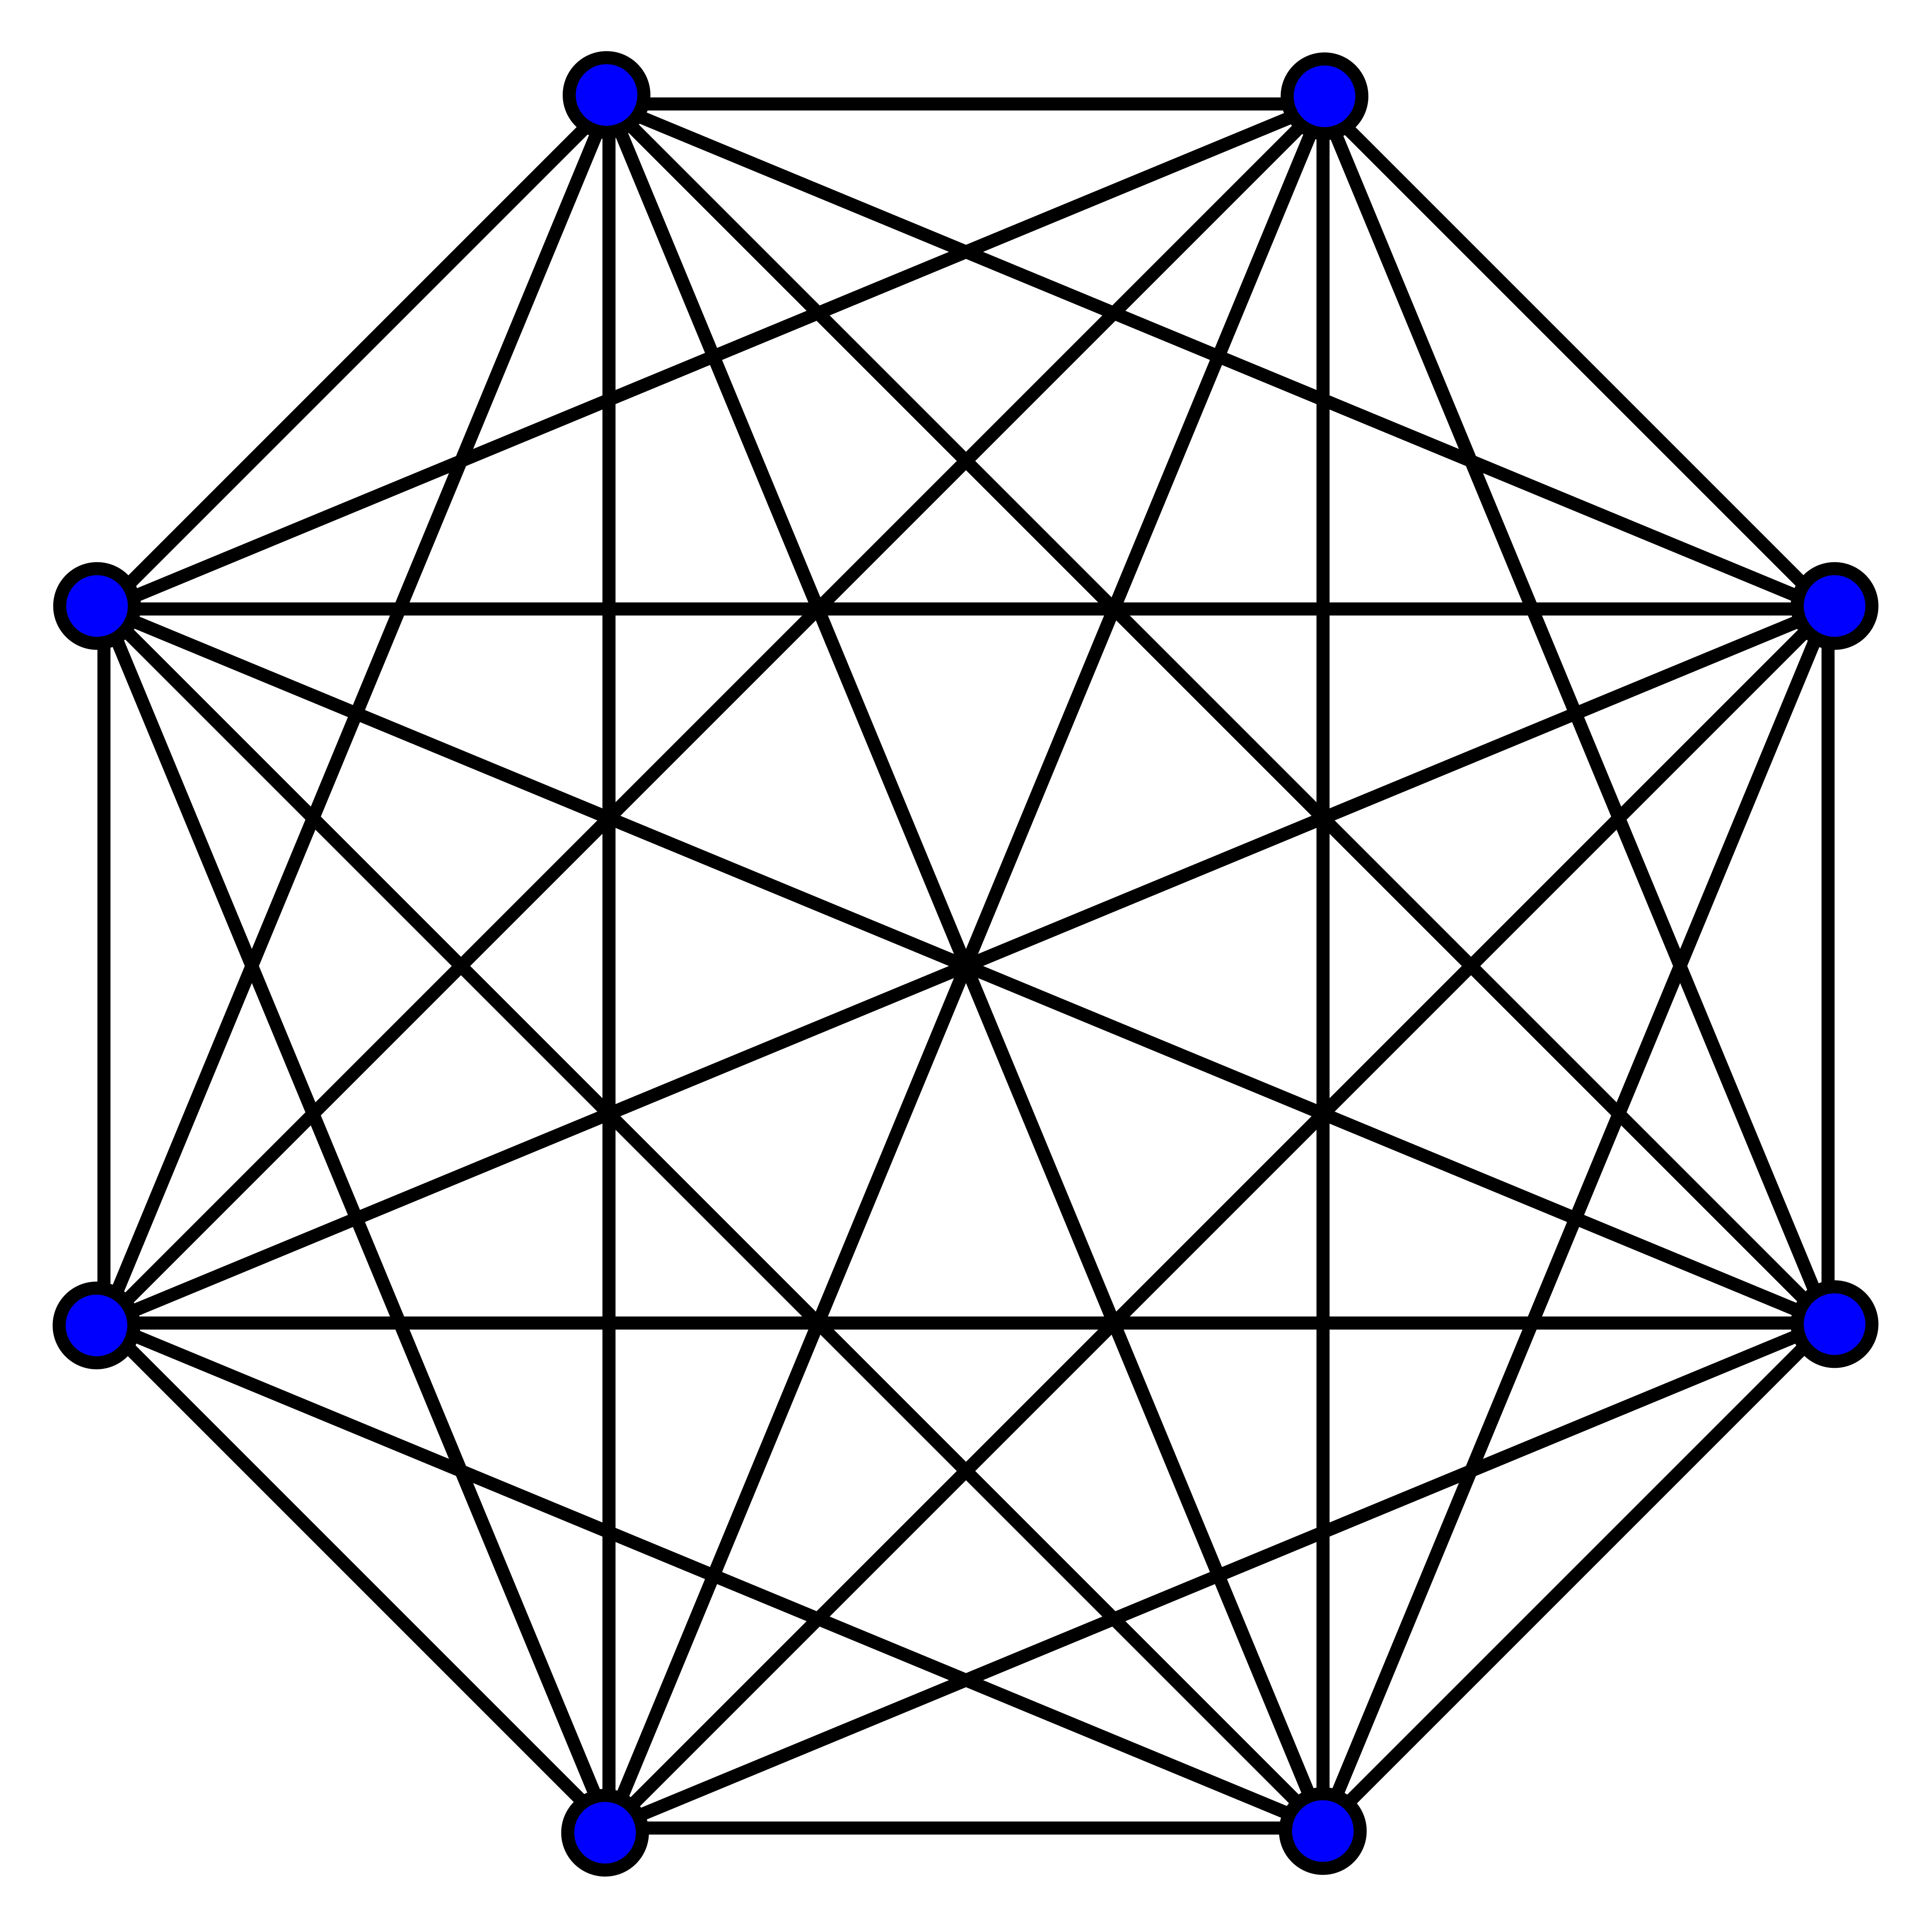
\includegraphics[width=0.3\textwidth]{comp_graph.png}
    \caption{Complete Graph}
    \label{}
\end{figure}
$$
H_{cost}=\sum_{i,j} d_{i,j} \hat p_{i,j}=\frac{1}{2}\sum_{i,j} d_{i,j} (I-Z_{i,j})
$$
Instead of encoding vertices as Hadfield did, here we encoding the edges of a TSP into the cost Hamiltonian. Where $\hat p_{i,j}=1/2(I-Z_{i,j})$ indicates wether the edge $(i,j)$ is chosen. Each edge in the graph is represented by a qubit.

$$
\begin{cases}
    \hat p_{i,j}=1 \text{ if edge (i,j) is chosen} \\
    \hat p_{i,j}=0 \text{ if edge (i,j) is not chosen}
\end{cases} 
$$

Eg.
$0\rightarrow3\rightarrow1\rightarrow2\rightarrow4$ is a solution for a 5 cities TSP,
in undirected conditions, it equals to 
$0\rightarrow4\rightarrow2\rightarrow1\rightarrow3$ which is the reverse of the previous solution.

$$
\begin{bmatrix}
    0&d_{0,1}&d_{0,2}&\hlight{d_{0,3}}&d_{0,4}&\\
    d_{1,0}&0&\hlight{d_{1,2}}&d_{1,3}&d_{1,4}&\\
    d_{2,0}&d_{2,1}&0&d_{2,3}&\hlight{d_{2,4}}&\\
    d_{3,0}&\hlight{d_{3,1}}&d_{3,2}&0&d_{3,4}&\\
    \hlight{d_{4,0}}&d_{4,1}&d_{4,2}&d_{4,3}&0&\\
\end{bmatrix}
\Leftrightarrow
\begin{bmatrix}
    0&d_{0,1}&d_{0,2}&d_{0,3}&\hlight{d_{0,4}}&\\
    d_{1,0}&0&d_{1,2}&\hlight{d_{1,3}}&d_{1,4}&\\
    d_{2,0}&\hlight{d_{2,1}}&0&d_{2,3}&0d_{2,4}&\\
    \hlight{d_{3,0}}&d_{3,1}&d_{3,2}&0&d_{3,4}&\\
    d_{4,0}&d_{4,1}&\hlight{d_{4,2}}&d_{4,3}&0&\\
\end{bmatrix}
$$

Since the setup of a TSP is completely determined by its distance matrix, containing $n(n-1)$ non zero elements, we just need the same number of qubits to encoding each edge of the graph. But it should be noticed that the encoding scheme reserves huge redundancy. The combination space for edge coding is $C_{n(n-1)}^n$, which is much larger than $A_{n-1}^{n-1}$. To form a circle requires in TSP, we need to pick $n$ edges, and add constraints that $\forall\, i\in S, deg(i)=2$, ensuring that each city is passed. 

We can use the same operator ansatz technique to preserve these constraints and compress the search space.

\section{Initial State}
The initial state must be a valid solution of TSP. Here we pick a simple situation. 
$$
|\psi_0\rangle=|\bar 0\rangle \otimes_{i=1}^{n-1} |1_{i,i+1}\rangle\otimes\bra{1_{n,0}}
$$

For example the $5\times 5$ matrix below.
$$
\begin{bmatrix}
    0&\hlight{d_{0,1}}&d_{0,2}&d_{0,3}&d_{0,4}&\\
    d_{1,0}&0&\hlight{d_{1,2}}&d_{1,3}&d_{1,4}&\\
    d_{2,0}&d_{2,1}&0&\hlight{d_{2,3}}&d_{2,4}&\\
    d_{3,0}&d_{3,1}&d_{3,2}&0&\hlight{d_{3,4}}&\\
    \hlight{d_{4,0}}&d_{4,1}&d_{4,2}&d_{4,3}&0&\\
\end{bmatrix}
$$
The ansatz is $\bra{0\rightarrow 1 \rightarrow 2\rightarrow 3\rightarrow 4}$, with cost $\sum_{i=0}^4 d_{i,i+1}$


\section{Mixer Hamiltonian}
The preserve the solution space, we must find the solution-transfer operator that transfer a valid solution into another one. In TSP, the most simple transfer operator is to swap the order of two cities (adjancent swap). Mathematically we can prove that the transfer between any two state in solution space can be decomposed into a series of adjancent swap operations. Thus a adjancent swap can be used as partial mixer in operator ansatz.

Denote $...u\rightarrow i \rightarrow j \rightarrow v\rightarrow...$ as $|u,i,j,v\rangle$, where $u, i, j, v$ are all cities. 
Define the partial mixer $H_{(u,v)(i,j)}$, where  $H_{(u,v)(i,j)} |u,i,j,v\rangle =|u,j,i,v\rangle$. Next step is to implement the adjancent swap with edge encoding. First noticed that the cost of $\bra{u,i,j,v}$ is $...+d_{u,i}+d_{i,j}+d_{j,v}+...$, and corresponding cost of $\bra{u,j,i,v}$ is $...+d_{u,j}+d_{j,i}+d_{i,v}+...$. In undirected graphs, since $d_{i,j}=d_{j,i}$, the swap can be wroten as following:
%  $$
%  H_{mixer}=\sum_{\{i,j\},\{u,v\}} S^-_{u,i}S^-_{i,j}S^-_{j,v}S^+_{u,j}S^+_{j,i}S^+_{i,v}+S^+_{u,i}S^+_{i,j}S^+_{j,v}S^-_{u,j}S^-_{j,i}S^-_{i,v}
%  $$
$$
H_{(u,v)(i,j)}= S^-_{u,i}S^-_{j,v}S^+_{u,j}S^+_{i,v}+S^+_{u,i}S^+_{j,v}S^-_{u,j}S^-_{i,v}
$$
where $S^+=|1\rangle\langle 0|=X+i Y$ and $S^-=|0\rangle\langle 1|=X-i Y$.
And the full mixer:
$$
H_{mixer}=\sum_{\{i,j\},\{u,v\}}H_{(u,v)(i,j)}
$$

\section{Circuit Optimization}
TBD
\section{Numerical Results}
TBD
\section{Discussion}
This encoding scheme is equivalent to the original operator ansatz, where at least $(n-1)^2$ qubits is needed. For the edge encoding, we need to map every non-zero matrix elements (one edge) to a qubit. Thus $n(n-1)$ qubits are required for a complete graph. But if we take the special situation where the TSP is undirected, the new encoding scheme will only requires $n(n-1)/2$ qubits since we can map index $\{i,j\}$ and $\{j,i\}$ to one same qubit, which represents one same edge. With this approach, the qubits needed for undirected TSP is reduced from $(n-1)^2$ to $n(n-1)/2$.


\bibliography{ref.bib}

\end{document}
%
% ****** End of file apssamp.tex ******